\section{Optimize Square Matrix-Matrix Multiplication  \punkte{50}}
\subsection{Implementation}
As given in the exercise, the optimal block size is
\begin{equation}
	s = \sqrt{\frac{M}{3}}
\end{equation}
where $M$ is the size of the fast memory. In our case this is the size of the L1 cache, which is 32KB as seen in table \ref{tab:cache}. In our dgemm-blocked implementation we use the double type, which has size 64 bit or 8 byte. Therefore we can convert our L1 cache size into bytes and divide it by the size of the double type in order to get $M$.
\begin{equation}
	M = \frac{32000}{8} = 4000 \ \text{doubles}
\end{equation}
After finding $M$, we can now calculate $s$:
\begin{equation}
	s = \sqrt{\frac{4000}{3}} = 36.5148 \approx 36 \ \text{blocks}
\end{equation}
We can now insert this result into the blocked dgemm code given in Listing \ref{lst:dgemm}.
Shifting our attention to the actual implementation of Blocked dgemm.
The goal is to improve cache utilization by optimizing the memory access pattern and reduce cache misses.\newline
The two outer loops split the matrix up into smaller blocks of the previously calculated block sizes $s$.
The next two inner loops go through the individual entry of each block and make sure if the final block cannot be completely filled due to the matrix dimension, that there's not an out-of-bounds error. The innermost loop iterates over the shared dimension.
Finally the computation is then performed according to the column-major format. 
Notice that an additional variable sum is introduced, which reduces the times we have to write to the C matrix.
\begin{lstlisting}[language=C++, caption=Dgemm blocked, label=lst:dgemm]
 const char *dgemm_desc = "Blocked dgemm.";

// Optimize for single core
#define BLOCK_SIZE 36

/* This routine performs a dgemm operation
 *
 *  C := C + A * B
 *
 * where A, B, and C are lda-by-lda matrices stored in column-major format.
 * On exit, A and B maintain their input values.
 */
void square_dgemm(int n, double *A, double *B, double *C) {
  double sum;
  for (int bi = 0; bi < n; bi += BLOCK_SIZE) {
    for (int bj = 0; bj < n; bj += BLOCK_SIZE) {
      for (int i = bi; i < bi + BLOCK_SIZE && i < n; i++) {
        for (int j = bj; j < bj + BLOCK_SIZE && j < n; j++) {
          sum = C[i + j * n];
          for (int k = 0; k < n; k++) {
            sum += A[i + k * n] * B[k + j * n];
          }
          C[i + j * n] = sum;
        }
      }
    }
  }
}
 \end{lstlisting}
This initial dgemm block implementation shows a significant improvement compared to the naive dgemm implementation as depicted in Figure \ref{fig:dgemm-0}
\begin{figure}[H]
	\centering
	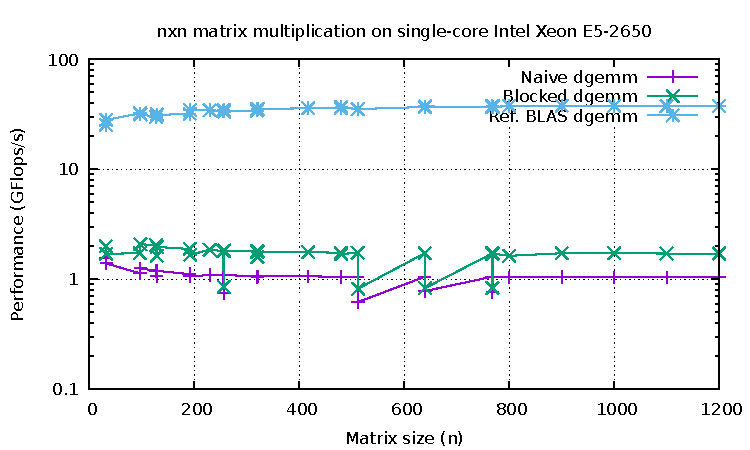
\includegraphics[width=\textwidth]{../media/timing-36.pdf}
	\caption{Timing of initial block matrix implementation}
	\label{fig:dgemm-0}
\end{figure}

\subsection{Unrolling Loops and Pragma statements}
As an attempt of improving the performance further, the innermost loop was replaced by the unrolled loop seen in Listing \ref{lst:unrolled}.
This loop is unrolled by a factor of 4, because this is equivalent to the number of doubles the FPU can process concurrently with a single SIMD instruction.
\begin{lstlisting}[language=C++, caption=Unrolled loop, label=lst:unrolled]
int k;
for (k = 0; k <= n - 4; k += 4) {
	sum += A[i + k * n] * B[k + j * n];
	sum += A[i + (k + 1) * n] * B[(k + 1) + j * n];
	sum += A[i + (k + 2) * n] * B[(k + 2) + j * n];
	sum += A[i + (k + 3) * n] * B[(k + 3) + j * n];
}
// For the final block if the number of elements is not divisible by 4
for (; k < n; k++) {
	sum += A[i + k * n] * B[k + j * n];
}
\end{lstlisting}
As a second approach the \texttt{\#pragma gcc ivdep} \cite{noauthor_loop-specific_nodate} directive was introduced in order to force the compiler to unconditionally vectorize the innermost loop.
Both approach did not show any improvement in performance compared to the initial block matrix implementation in Figure \ref{fig:dgemm-0}.
Hence these approaches were subsequently removed from my final blocked dgemm implementation, but the output file for this option can be found in the submission.
These approaches were most likely unsuccessful due to the compiler being able of doing these optimization on its own. This theory is reinforced by having a look at the provided compiler flags in the \texttt{Makefile} this includes flags such as \texttt{-funroll-loops} and \texttt{-march=native}.

\subsection{Compiler Flags}
By introducing further compiler flags, it is possible to increase the performance even more. Especially the addition of \texttt{-ffast-math} \cite{noauthor_floatingpointmath_nodate} resulted in an significant uptick in performance, see Figure \ref{fig:dgemm-fm}. It enables a set of flag that enables aggressive floating-point optimizations, but be aware \texttt{-ffast-math} is not always safe.
\begin{figure}[H]
	\centering
	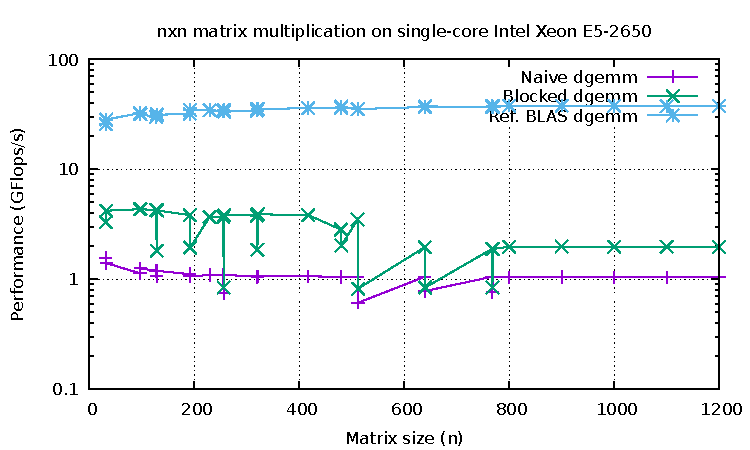
\includegraphics[width=\textwidth]{../media/timing-36-fast-math.pdf}
	\caption{Timing of dgemm using ffast-math}
	\label{fig:dgemm-fm}
\end{figure}


